\documentclass{article}

\usepackage{subcaption}
\usepackage[utf8]{inputenc}
\usepackage[english]{babel}
\usepackage[backend=bibtex]{biblatex}
\usepackage{tikz}
\usepackage{xcolor}
\usepackage{multicol}
\usepackage{listings}
\usepackage{csquotes}
\usepackage[most]{tcolorbox}
\usepackage{parskip}
\usepackage{listings-rust}
\usepackage[scale=0.9]{sourcecodepro}
\usepackage{bytefield}
\usepackage{tikz}
\usepackage{adjustbox}
\usepackage{float}

\addbibresource{ref}


\usetikzlibrary{arrows, automata, positioning}

\usepackage[a4paper, total={6in, 8in}]{geometry}

\tcbset {
  base/.style={
    arc=0mm,
    bottomtitle=0.5mm,
    boxsep=1mm,
    boxrule=0mm,
    colbacktitle=black!10!white,
    coltitle=black,
    fonttitle=\bfseries,
    left=2.5mm,
    leftrule=1mm,
    right=3.5mm,
    title={#1},
    toptitle=0.75mm,
  },
    sub/.style={
        base={#1},
        colframe=black!30!white,
        top=-0.5mm,
        bottom=-0.5mm,
    },
}

\definecolor{brandblue}{rgb}{0.34, 0.7, 1}
\newtcolorbox{mainbox}[1]{
    nobeforeafter,
    colframe=brandblue,
    base={#1}
}

\newtcolorbox{subbox}[1]{
  colframe=black!30!white,
  sub={#1}
}

\newtcolorbox{warningbox}[1]{
  colframe=red,
  base={#1}
}

\usepackage{lato}
\renewcommand*\familydefault{\sfdefault}
\newcommand{\code}[1]{\texttt{#1}}
\usepackage[T1]{fontenc}
\usepackage{hyperref}
\usepackage{fancyhdr}

\pagestyle{fancy}
\fancyhf{}
\rhead{Giorgio Grigolo}
\lhead{CPS 2000: Compiler Theory and Practice}
\rfoot{Page \thepage}

\definecolor{bluekeywords}{rgb}{0.13, 0.13, 1}
\definecolor{greencomments}{rgb}{0, 0.5, 0}
\definecolor{redstrings}{rgb}{0.9, 0, 0}
\definecolor{graynumbers}{rgb}{0.5, 0.5, 0.5}


\lstset{
    commentstyle=\color{greencomments},
    keywordstyle=\color{bluekeywords},
    stringstyle=\color{redstrings},
    numberstyle=\color{graynumbers},
    % breaklines=true,
    basicstyle=\ttfamily,
    language=Rust,
    xleftmargin=.3\textwidth, xrightmargin=.3\textwidth,
    captionpos=b
}

\title{Compiling \code{ParL} to \code{PArIR} in Rust \\{\normalsize A report on the Rust
compiler for the \code{ParL} programming language.}}
\author{Giorgio Grigolo - 0418803L}
\date{}

\hypersetup{
    colorlinks=true,
    linkcolor=blue,
    filecolor=magenta,
    urlcolor=blue,
}

\begin{document}

\maketitle
\tableofcontents

\begin{abstract}
    In this report, we discuss the implementation details of a
    compiler for \code{ParL}, an expression-based strongly typed programming
    langauge. Code written in \code{ParL} is compiled to \code{PArIR}, which is
    the proprietary assembly-like language that is used to drive the
    programmable pixel art displays designed by the company \code{PArDis}. The
    \code{ParL} compiler was written in Rust, due to its strong type system and
    performance characteristics. It was implemented incrementally, as
    to ensure each component can be run in isolation, and is working correctly
    before moving on to the next one.
\end{abstract}

\newpage

\section{Project Structure}

\newpage

\section{Lexical Analysis}

The first step in the compilation process is the lexical analysis. A recurring
theme in the implementation of this compiler is the use of \textit{abstraction}
to achieve \textit{modularity}, and simplify the implementation of the
subsequent stages. The lexical analysis is no exception to this rule.

At the highest level, the lexical analysis is implemented as a \code{Lexer}
struct, which is responsible for reading the input source code, and producing a
stream (\textit{or vector}) of tokens.

We shall start by defining the \code{Token} struct, which is a wrapper for the
different types of tokens that can be found in a \code{ParL} program. The
\code{Token} enum is defined as follows:

\begin{mainbox}{}
    \lstset{belowskip=0pt, aboveskip=0pt}
    \begin{lstlisting}
pub struct Token {
    pub kind: TokenKind,
    pub span: TextSpan,
}
    \end{lstlisting}
\end{mainbox}

The \code{TextSpan} struct is mainly used to store the lexeme of the token, and
its position in the source code, which is useful for error reporting. The
\code{TokenKind} is just an enum, which represents the different types of tokens, such as \code{Identifier},
\code{IntegerLiteral}, \code{If} and many more.


The actual \code{Lexer} struct is defined as follows:

\begin{mainbox}{}
    \lstset{belowskip=0pt, aboveskip=0pt}
    \begin{lstlisting}[caption={The \code{Lexer} struct.}]
pub struct Lexer<B: Stream> {
    buffer: B,
    dfsa: Dfsa,
}
    \end{lstlisting}
\end{mainbox}

The \code{Lexer} struct is generic over the type \code{B}, which is a trait that
abstracts out the file reading logic from the lexer. This is useful for testing
purposes, as we can easily mock the file reading logic, and test the lexer in
isolation. It is also useful in case the lexer is to be improved in the future,
by using more efficient file reading logic, such as the double buffering
technique.

The main function of the \code{Lexer} struct is the \code{next\_token} function,
which is responsible for reading the next token from the input stream. Not much
can be said, as it has been heavily inspired by the \code{next\_token} function
in the textbook \textit{Engineering a Compiler} \cite{engineering-a-compiler}.
We provide a wrapper around the \code{next\_token} function, called
\code{lex()}, which filters out comments, whitespace and newlines, and only
returns the actual tokens, and if any, a list of errors that have been
encountered.


We note that the \code{next\_token} returns \code{Result<Token, LexicalError>}
instead of just a \code{Token}, which is caught by the wrapper \code{lex()}.
This feature, known as \textit{synchronization} allows the lexer to return an
error, instead of crashing. This enables the lexer to recover after an error has
been encountered, such as reading a character that is not in the character table
of the DFSA. It will continue reading from the next token, and find other
invalid characters.

\begin{center}
    \textit{Whilst using a compiler, one would expect to
        be given as many errors as possible, instead of
        playing whack-a-mole with the compiler.}
\end{center}

\newpage

\subsection{DFSA Builder}

Of course, the \code{Lexer} that was implemented in the project, was required to
be a based on a finite state automaton, with a character table. Initially, the
DFSA was implemented manually, but as the number of tokens (and hence states)
grew it was getting harder to keep track of the transitions.

To solve this problem, together with the \code{Dfsa} struct, a
\code{DfsaBuilder} struct was implemented, which is responsible for dynamically
building the DFSA from a number of chained function calls. I will describe each
method of the \code{DfsaBuilder} struct, and how it is used, by demonstrating
the effect as it is run incrementally on an empty DFSA.


The \code{DfsaBuilder} struct is defined as follows:

\begin{mainbox}{}
    \lstset{xleftmargin=0cm}
    \begin{lstlisting}
pub struct DfsaBuilder {
    pub max_state: i32,
    pub accepted_states: Vec<i32>,
    pub character_table: HashMap<char, Category>,
    pub transition_table: HashMap<(i32, Category), i32>,
    pub state_to_token: HashMap<i32, TokenKind>,
}
    \end{lstlisting}
\end{mainbox}

Clearly, we can see that states are represented by \code{i32} integers, and
transitions are represented by a tuple of the current state and the category of
the character that is being read. The category of a character is defined by the
\code{Category} enum, containing variants such as \code{Digit}, \code{Letter},
\code{Whitespace}, and many more.


The first function is $$\code{add\_category(\&mut self, range: Vec<char>,
        category: Category)}$$  This method is used to add multiple characters to the
same category.  For example, we can add all the digits to the \code{Digit}
category, by calling \code{add\_category('0'..='9', Category::Digit)}. Note that
in the actual implementation, the \code{range} parameter is actually a more
complex type, but for simplicity's sake it can be thought of a vector. It
actually accepts anything that can be casted to an iterator, as to allow for
more convenient usage. This is done using Rust's built in ranges like
\code{'0'..='9'}. As it does not have any effect on the DFSA, but only modifies
the character table, a DFSA will not be shown.

Then, we have $$\code{add\_transition(\&mut self, state: i32, category:
        Category, next\_state: i32)}$$ This method is used to add a transition from one
state to another, given a category. For example, we can add a transition from
state 0 to state 1, when reading a digit, by calling \code{add\_transition(0,
    Category::Digit, 1)}. Note that it doesn't automatically make the state 1 an
accepted state, as it is only responsible for adding transitions.


\begin{figure}[H]
    \begin{subfigure}[t]{0.5\textwidth}
        \centering
        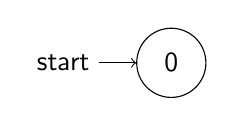
\begin{tikzpicture}
            \node[state, initial] (0) {0};
        \end{tikzpicture}
        \caption{The DFSA before adding calling \code{add\_transition}}
    \end{subfigure}
    \begin{subfigure}[t]{0.5\textwidth}
        \centering
        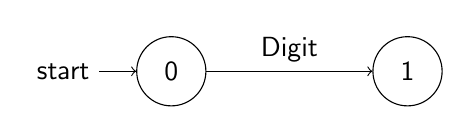
\begin{tikzpicture}
            \node[state, initial] (0) {0};
            \node[state, right of=0, xshift=2cm] (1) {1};
            \draw (0) edge[above, ->] node{Digit} (1);
        \end{tikzpicture}

        \caption{The DFSA after adding calling \code{add\_transition}}
    \end{subfigure}
\end{figure}

The next function is $$\code{auto\_add\_transition(\&mut self, state: i32,
        category: Category}$$
$$\code{to: Option<i32>, token\_kind: TokenKind) -> i32}$$

This method is used used to add a transition from \code{(state, category)} to
the state \code{to}. Since \code{to} is an \code{Option}, it can be \code{None},
in which case the destination state is automatically set to the next state. This
is useful for adding transitions to the same state, as well as constructing
slightly more complicated sequences of transitions, say for tokenizing a float.
The \code{token\_kind} parameter is used to set the token kind of the state, if
it is an accepted state. Similarly to the \code{to} parameter, it can be
\code{None}, in which case the destination state is not an accepted state.  We
also note that this function returns an integer, which is the state that was
just added, for further use in subsequent calls.

If we run \code{auto\_add\_transition(2, Category::Digit, None, Category::Float)}, the resultant DFSA will be as follows:

\begin{figure}[H]
    \begin{subfigure}[t]{0.5\textwidth}
        \centering
        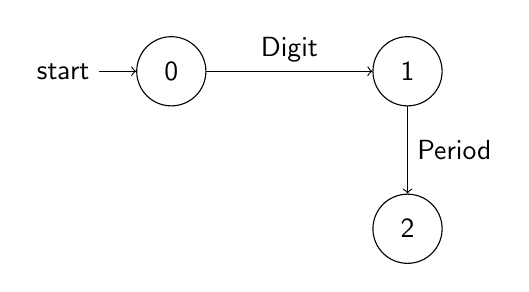
\begin{tikzpicture}
            \node[state, initial] (0) {0};
            \node[state, right of=0, xshift=2cm] (1) {1};
            \node[state, below of=1, yshift=-1cm] (2) {2};

            \draw (0) edge[above, ->] node{Digit} (1)
            (1) edge[right, ->] node{Period} (2);
        \end{tikzpicture}
        \caption{Before running the function}
    \end{subfigure}
    \begin{subfigure}[t]{0.5\textwidth}
        \centering
        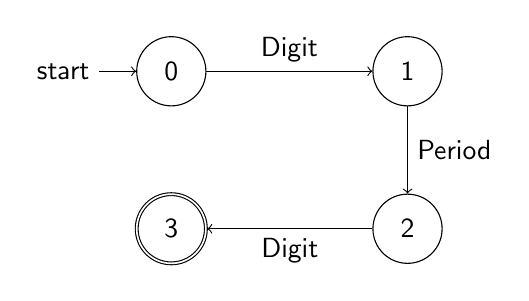
\begin{tikzpicture}
            \node[state, initial] (0) {0};
            \node[state, right of=0, xshift=2cm] (1) {1};
            \node[state, below of=1, yshift=-1cm] (2) {2};
            \node[state, accepting, below of=0, yshift=-1cm] (3) {3};

            \draw (0) edge[above, ->] node{Digit} (1)
            (1) edge[right, ->] node{Period} (2)
            (2) edge[below, ->] node{Digit} (3);
        \end{tikzpicture}
        \caption{After running the function}
    \end{subfigure}
\end{figure}

If we run \code{auto\_add\_transition(2, Category::Digit, Some(5), None)}, the
resultant DFSA will be as follows, meaning we just want to map to an auxiliary
state that doesn't correspond to any token kind, (and thus is not an accepted
state), the following is the resulting DFSA.

\begin{figure}[H]
    \begin{subfigure}[t]{0.5\textwidth}
        \centering
        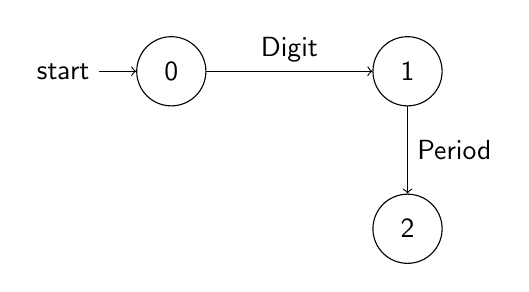
\begin{tikzpicture}
            \node[state, initial] (0) {0};
            \node[state, right of=0, xshift=2cm] (1) {1};
            \node[state, below of=1, yshift=-1cm] (2) {2};

            \draw (0) edge[above, ->] node{Digit} (1)
            (1) edge[right, ->] node{Period} (2);
        \end{tikzpicture}
    \end{subfigure}
    \begin{subfigure}[t]{0.5\textwidth}
        \centering
        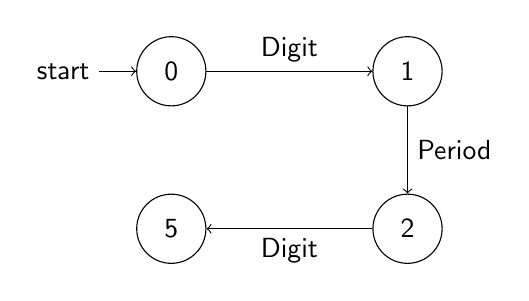
\begin{tikzpicture}
            \node[state, initial] (0) {0};
            \node[state, right of=0, xshift=2cm] (1) {1};
            \node[state, below of=1, yshift=-1cm] (2) {2};
            \node[state, below of=0, yshift=-1cm] (3) {5};

            \draw (0) edge[above, ->] node{Digit} (1)
            (1) edge[right, ->] node{Period} (2)
            (2) edge[below, ->] node{Digit} (3);

        \end{tikzpicture}
    \end{subfigure}
\end{figure}

Next up, we have the function

\begin{center}
    \code{add\_final\_character\_symbol(character: char, category: Category, token\_kind: TokenKind)}
\end{center}

This function is a shortcut for adding single characters that are final symbols,
such as the semicolon, or the period to the character table, and the transition
that follows from this to the transitions table.

Suppose we called \code{add\_final\_character\_symbol(';',
    Category::Semicolon,} \\ \code{TokenKind::Semicolon)}. The resultant DFSA would
be as follows:

\begin{figure}[H]
    \begin{subfigure}[t]{0.5\textwidth}
        \centering
        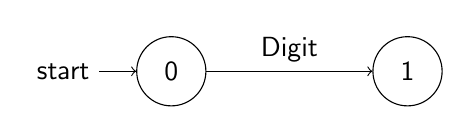
\begin{tikzpicture}
            \node[state, initial] (0) {0};
            \node[state, right of=0, xshift=2cm] (1) {1};

            \draw (0) edge[above, ->] node{Digit} (1);
        \end{tikzpicture}
    \end{subfigure}
    \begin{subfigure}[t]{0.5\textwidth}
        \centering
        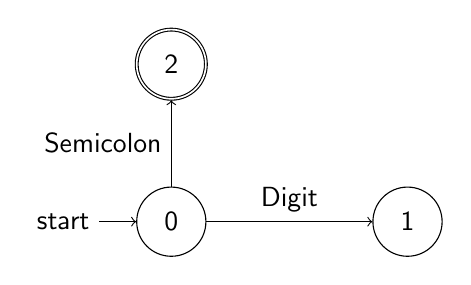
\begin{tikzpicture}
            \node[state, initial] (0) {0};
            \node[state, right of=0, xshift=2cm] (1) {1};
            \node[state, accepting, above of=0, yshift=1cm] (2) {2};

            \draw (0) edge[above, ->] node{Digit} (1)
            (0) edge[left, ->] node{Semicolon} (2);
        \end{tikzpicture}
    \end{subfigure}
\end{figure}

Then we have a function that does the same thing as the previous one, but is
able to take in multiple tuples of the type (\code{char}, \code{Category},
\code{TokenKind}), and add them all at once. This function is called
\code{add\_final\_character\_symbols}.

Finally, we have the function \code{build}, which is used to build the DFSA from the builder. This function is called at the end of the chain of function calls, and returns the DFSA that was built.

\begin{center}
    \rule{0.5\textwidth}{0.4pt}
\end{center}

Clearly, the \code{DfsaBuilder} has proved itself useful for an efficient and
readable way to build the DFSA for the lexer. However, we still require a
greater degree of freedom when it comes to making complex multi-character
transitions.

\begin{warningbox}{}
    In the production rules for the \code{ParL} grammar, there is a slight
    inconsistency. There is an overlap between the \code{Letter} and the
    \code{Hex} symbol. This was taken into account by creating an auxiliary
    category called \code{HexAndLetter}, so that the lexer can differentiate
    between the two.
\end{warningbox}

To be able to get around the above inconsistency, as well as to allow for the
aforementioned flexibility, we can also call the \code{.transition()} method on
the \code{DfsaBuilder}, and have it return an instance of the \code{Transition}
struct. This transition automatically starts from the first unused state index,
(which is kept track of in the \code{max\_state} member of the
\code{DfsaBuilder} struct) and gives us another set of functions we can chain to
further build the transition.

The \code{Transition} struct holds a reference to the \code{DfsaBuilder} that it
was created from, the current state, the list of transitions that have been
added, and the a list of final states with the token kind that they return.

\begin{mainbox}{}
    \lstset{xleftmargin=1cm}
    \begin{lstlisting}
pub struct Transition<'a> {
    dfsa_builder: &'a mut DfsaBuilder,
    current_state: i32,
    transitions: Vec<((Category, i32), i32)>,
    final_state_token: Vec<(i32, TokenKind)>,
}
    \end{lstlisting}
\end{mainbox}


The first function that can be called on the \code{Transition} struct is the following:
$$\code{to(category: Category) -> Transition}$$

This method is used to just append a single category to the transition. Calling
it multiple times, increments an internal pointer, that always points to the
last state that was added. Thus, calling it multiple times creates a
\textit{chain} of states.


\begin{figure}[H]
    \begin{subfigure}[t]{0.5\textwidth}
        \centering
        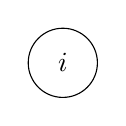
\begin{tikzpicture}
            \node[state] (0) {$i$};
        \end{tikzpicture}
        \caption{The transition before adding calling \code{to}}
    \end{subfigure}
    \begin{subfigure}[t]{0.5\textwidth}
        \centering
        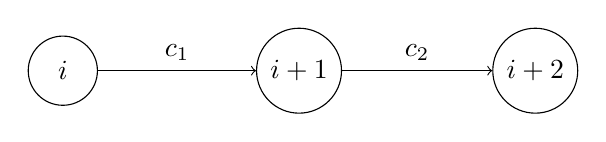
\begin{tikzpicture}
            \node[state] (0) {$i$};
            \node[state, right of=0, xshift=2cm] (1) {$i+1$};
            \node[state, right of=1, xshift=2cm] (2) {$i+2$};
            \draw (0) edge[above, ->] node{$c_1$} (1);
            \draw (1) edge[above, ->] node{$c_2$} (2);
        \end{tikzpicture}
        \caption{The transition after adding calling \code{to} twice with $c_1$ and $c_2$ respectively}
    \end{subfigure}
\end{figure}


Then, we have the $\code{repeated()}$ method, which is used to allow an
indeterminate number of repetitions of the last category, think of this as the
\code{*} symbol in regular expressions.

\begin{figure}[H]
    \begin{subfigure}[t]{0.5\textwidth}
        \centering
        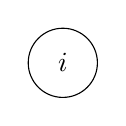
\begin{tikzpicture}
            \node[state] (0) {$i$};
        \end{tikzpicture}
        \caption{The transition before adding calling \code{repeated}}
    \end{subfigure}
    \begin{subfigure}[t]{0.5\textwidth}
        \centering
        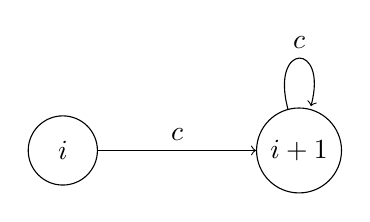
\begin{tikzpicture}
            \node[state] (0) {$i$};
            \node[state, right of=0, xshift=2cm] (1) {$i+1$};
            \draw (0) edge[above, ->] node{$c$} (1);
            \draw (1) edge[above, ->, loop above] node{$c$} (1);
        \end{tikzpicture}
        \caption{The transition after adding calling \code{to(c)} followed by  \code{repeated()}}
    \end{subfigure}
\end{figure}


Whenever we want to make the last state an accepted state, we can thenc all the
$$\code{goes\_to(token\_kind: TokenKind)}$$ method, that simply marks the last state as
an accepted state, and sets the token kind it returns to the one that was passed
as an argument.

Finally, we have the $\code{done()}$ method, which is used to append the transition that has been prepared to the actual DFSA from which \code{.transition()} was called from.


\begin{mainbox}{}
    \lstset{xleftmargin=1cm, aboveskip=0pt, belowskip=0pt}
    \begin{lstlisting}
        let mut builder = DfsaBuilder::new();
        builder.add_category([' '], ['\t'], Category::Whitespace)
               .transition()
               .to([Category::Whitespace])
               .repeated()
               .goes_to(TokenKind::Whitespace)
               .done();
    \end{lstlisting}
\end{mainbox}

Would result in the following DFSA, with the category table already filled in
with the whitespace characters.

\begin{figure}[H]
    \centering
    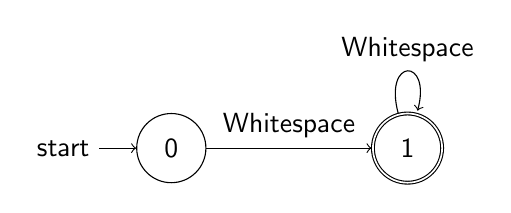
\begin{tikzpicture}
        \node[state, initial] (0) {0};
        \node[state, accepting, right of=0, xshift=2cm] (1) {1};

        \draw (0) edge[above, ->] node{Whitespace} (1);
        \draw (1) edge[above, ->, loop above] node{Whitespace} (1);
    \end{tikzpicture}
\end{figure}

The actual definitions of the DFSA that was used in the lexer can be found in
\code{lexer.rs}, as part of the \code{Lexer::new()} function, and also in
Appendix \ref{sec:lexer-dfsa}.


\newpage

\section{Parsing}

\newpage



\appendix

\section{Lexer DFSA}
\label{sec:lexer-dfsa}

\begin{mainbox}{}
    \lstset{xleftmargin=0cm}
    \begin{lstlisting}
    pub fn new(input: &str, file: &Path, dfsa: Option<Dfsa>) -> Self {
        let mut dfsa_builder = DfsaBuilder::new();

        match dfsa {
            Some(dfsa) => Lexer {
                buffer: B::new(input, file),
                dfsa,
            },
            None => {
                let dfsa = dfsa_builder
                    .add_category('a'..='f', Category::HexAndLetter)
                    .add_category('A'..='F', Category::HexAndLetter)
                    .add_category('g'..='z', Category::Letter)
                    .add_category('G'..='Z', Category::Letter)
                    .add_category('0'..='9', Category::Digit)
                    .add_final_character_symbols(vec![
                        ('\n', Category::Newline, TokenKind::Newline),
                        ('{', Category::LBrace, TokenKind::LBrace),
                        ('}', Category::RBrace, TokenKind::RBrace),
                        ('(', Category::LParen, TokenKind::LParen),
                        (')', Category::RParen, TokenKind::RParen),
                        ('[', Category::LBracket, TokenKind::LBracket),
                        (']', Category::RBracket, TokenKind::RBracket),
                        (';', Category::Semicolon, TokenKind::Semicolon),
                        (':', Category::Colon, TokenKind::Colon),
                        ('+', Category::Plus, TokenKind::Plus),
                        ('*', Category::Asterisk, TokenKind::Multiply),
                        (',', Category::Comma, TokenKind::Comma),
                        ('\0', Category::Eof, TokenKind::EndOfFile),
                        ('%', Category::Percent, TokenKind::Mod),
                    ])
                    .add_whitespace_logic()
                    .add_comment_functionality()
                    .add_multi_char_rel_ops()
                    .add_identifier_logic()
                    .add_number_logic()
                    .build();

                Lexer {
                    buffer: B::new(input, file),
                    dfsa,
                }
            }
        }
    }
    \end{lstlisting}
\end{mainbox}

\section{Parser AST Node Enum}
\label{sec:parser-ast-node-enum}

\begin{mainbox}{}
    \lstset{xleftmargin=0cm}
    \begin{lstlisting}
pub type AstNodePtr = Box<AstNode>;

#[derive(Debug)]
pub enum AstNode {
    Program {
        statements: Vec<AstNode>,
    },
    VarDec {
        identifier: Token,
        r#type: Token,
        expression: AstNodePtr,
    },
    Block {
        statements: Vec<AstNode>,
    },
    Expression {
        casted_type: Option<Token>,
        expr: AstNodePtr,
    },
    SubExpression {
        bin_op: AstNodePtr,
    },
    UnaryOp {
        operator: Token,
        expr: AstNodePtr,
    },
    BinOp {
        left: AstNodePtr,
        operator: Token,
        right: AstNodePtr,
    },
    PadWidth,
    PadRandI {
        upper_bound: AstNodePtr,
    },
    PadHeight,
    PadRead {
        x: AstNodePtr,
        y: AstNodePtr,
    },
    \end{lstlisting}
\end{mainbox}
\newpage
\begin{mainbox}{}
    \lstset{xleftmargin=0cm}
    \begin{lstlisting}
    IntLiteral(Token),
    FloatLiteral(Token),
    BoolLiteral(Token),
    ColourLiteral(Token),
    FunctionCall {
        identifier: Token,
        args: Vec<AstNode>,
    },
    ActualParams {
        params: Vec<AstNode>,
    },
    Delay {
        expression: AstNodePtr,
    },
    Return {
        expression: AstNodePtr,
    },
    PadWriteBox {
        loc_x: AstNodePtr,
        loc_y: AstNodePtr,
        width: AstNodePtr,
        height: AstNodePtr,
        colour: AstNodePtr,
    },
    PadWrite {
        loc_x: AstNodePtr,
        loc_y: AstNodePtr,
        colour: AstNodePtr,
    },
    Identifier {
        token: Token,
    },
    If {
        condition: AstNodePtr,
        if_true: AstNodePtr,
        if_false: Option<AstNodePtr>,
    },
    For {
        initializer: Option<AstNodePtr>,
        condition: AstNodePtr,
        increment: Option<AstNodePtr>,
        body: AstNodePtr,
    },
    While {
        condition: AstNodePtr,
        body: AstNodePtr,
    },

    \end{lstlisting}
\end{mainbox}

\begin{mainbox}{}
    \lstset{xleftmargin=0cm}
    \begin{lstlisting}

    FormalParam {
        identifier: Token,
        param_type: Token,
        index: Option<Token>,
    },
    FunctionDecl {
        identifier: Token,
        params: Vec<AstNode>,
        return_type: Type,
        block: AstNodePtr,
    },
    Print {
        expression: AstNodePtr,
    },
    Assignment {
        identifier: Token,
        expression: AstNodePtr,
        index: Option<AstNodePtr>,
    },
    PadClear {
        expr: AstNodePtr,
    },
    VarDecArray {
        identifier: Token,
        element_type: Token,
        size: usize,
        elements: Vec<AstNode>,
    },
    ArrayAccess {
        identifier: Token,
        index: AstNodePtr,
    },
    EndOfFile,
}
    \end{lstlisting}
\end{mainbox}

\newpage

\printbibliography


\end{document}
